\chapter{Manual de usuario de BreachLab}
\label{anexo:manual}

\section*{Introducción}

Este anexo describe, pantalla a pantalla, el funcionamiento de \breachlab
desde el punto de vista de un usuario de la aplicación.

\section{Pantalla de inicio de sesión}

Formulario de usuario y contraseña. Un panel lateral recuerda los usuarios
de prueba y permite reiniciar la base de datos para partir de
un estado limpio antes de una prueba.

\begin{figure}[H]
  \centering
  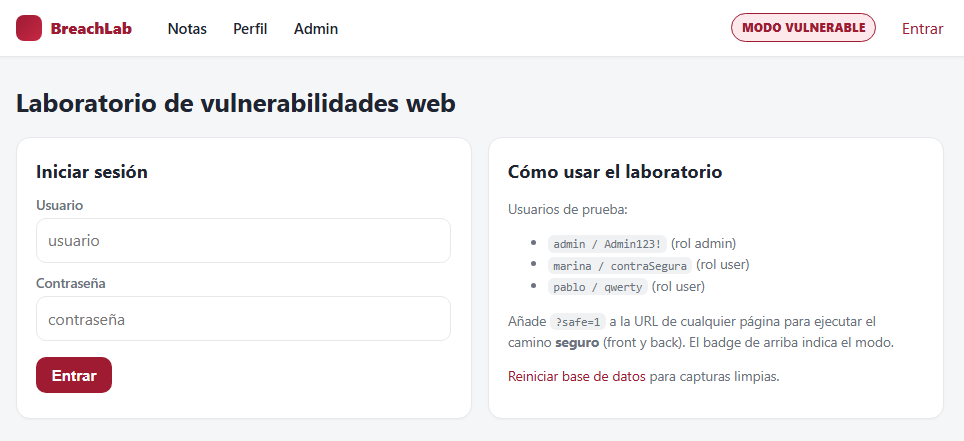
\includegraphics[width=0.85\textwidth]{figures/login.png}
  \caption{Pantalla de inicio de sesión de \breachlab.}
  \label{fig:anexo-login}
\end{figure}

\section{Dashboard y notas}

Tras iniciar sesión, el panel principal permite crear notas y listar las
propias, así como abrir cualquier nota por su identificador. En modo
vulnerable no se restringe el acceso a notas de otros usuarios (véase el
apartado~\ref{sec:idor}); en modo seguro (\texttt{?safe=1}) sí se restringe.

\begin{figure}[H]
  \centering
  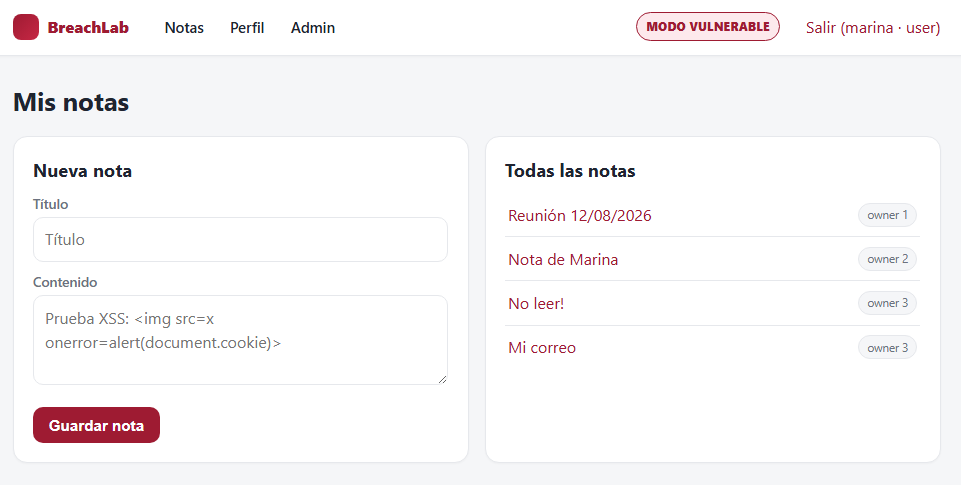
\includegraphics[width=0.85\textwidth]{figures/dashboard.png}
  \caption{Dashboard de notas, con el formulario de creación a la izquierda
    y el listado de todas las notas del sistema a la derecha.}
  \label{fig:anexo-dashboard}
\end{figure}

\section{Perfil}

Permite cambiar la contraseña del usuario autenticado. En modo seguro, el
formulario incluye el token CSRF obtenido de \texttt{GET /api/me}; en modo
vulnerable, el cambio de contraseña también puede forzarse desde un sitio
externo (véase \texttt{csrf\_poc.html} y el apartado~\ref{sec:csrf}).

\begin{figure}[H]
  \centering
  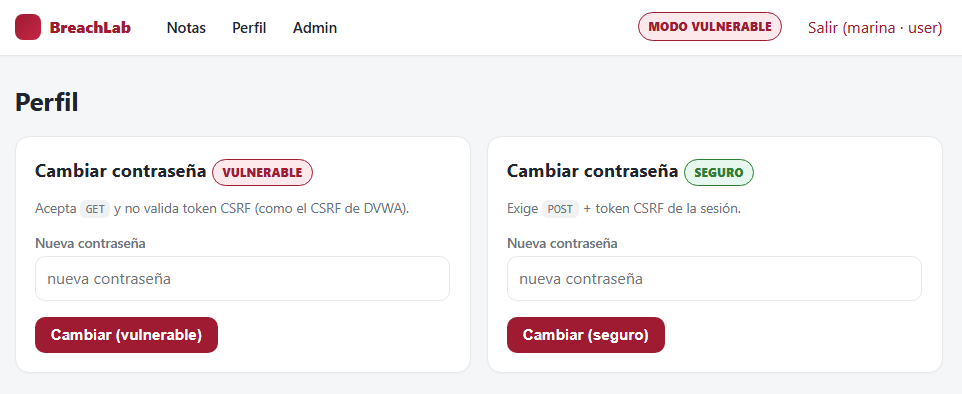
\includegraphics[width=0.85\textwidth]{figures/perfil.png}
  \caption{Pantalla de Perfil, con los dos formularios de cambio de
    contraseña —vulnerable y seguro— lado a lado.}
  \label{fig:anexo-perfil}
\end{figure}

\section{Panel de administración}

Muestra el listado completo de usuarios, incluidas sus contraseñas. En modo
vulnerable es accesible por cualquier usuario autenticado, no solo por
administradores (véase el apartado~\ref{sec:idor}); en modo seguro responde 403 si el
rol no es admin.

\begin{figure}[H]
  \centering
  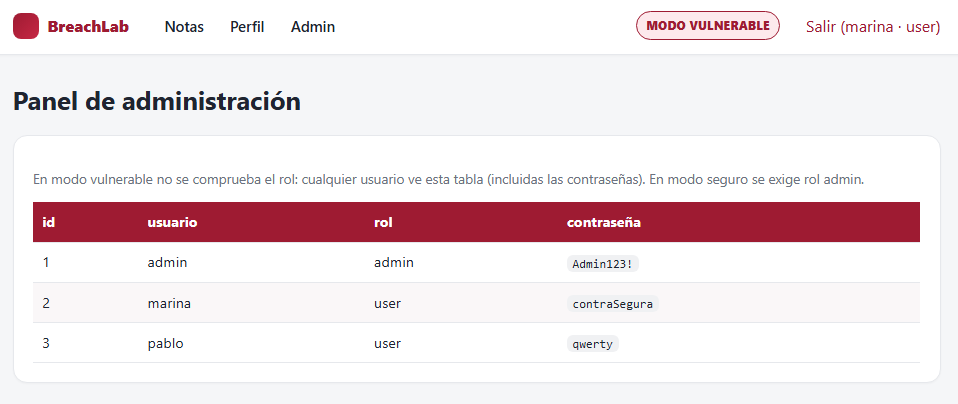
\includegraphics[width=0.75\textwidth]{figures/admin-vulnerable.png}
  \caption{Panel de administración en modo vulnerable: contraseñas visibles
    para cualquier usuario autenticado.}
  \label{fig:anexo-admin-vulnerable}
\end{figure}

\begin{figure}[H]
  \centering
  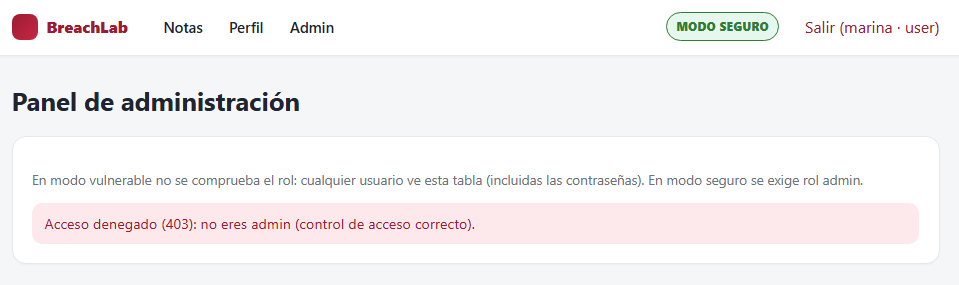
\includegraphics[width=0.75\textwidth]{figures/admin-seguro.png}
  \caption{El mismo panel en modo seguro: acceso denegado (403) por no
    tener rol \texttt{admin}.}
  \label{fig:anexo-admin-seguro}
\end{figure}

\section{Modo seguro (\texttt{?safe=1})}

Añadido a la URL de cualquier pantalla, un badge visible en la cabecera
indica que las contramedidas de todas las vulnerabilidades están activas,
tanto en el frontend como en el backend: «MODO VULNERABLE» en rojo por
defecto, «MODO SEGURO» en verde con \texttt{?safe=1}, visible en todas las
capturas anteriores.
